\documentclass{article}
\usepackage[preprint]{neurips_2026}
\usepackage[T1]{fontenc}
\usepackage{booktabs}
\usepackage{graphicx}
\usepackage{microtype}
\usepackage[margin=0pt,font=small,labelfont=bf,skip=2pt]{caption}
\graphicspath{{failures/}}
\setlength{\abovecaptionskip}{2pt}
\setlength{\belowcaptionskip}{0pt}
\setlength{\parskip}{0pt}
\captionsetup[table]{skip=3pt}

\title{Where Vision--Language Models Fail at 3D Space:\\A VSI-Bench Evaluation of Three Open-Weight VLMs}

\author{Noah Lee\\Texas A\&M University}

\raggedbottom
\begin{document}
\small
\maketitle
\vspace{-14mm}

\section{Setup and protocol}
We evaluate three open-weight VLMs on VSI-Bench~\citep{yang2025thinking}, 1316 questions over
288 egocentric scenes from ScanNet and ScanNet++. Every model receives the same input: 32 frames
sampled at $\mathrm{round}(\mathrm{linspace}(0,N{-}1,32))$, long side capped at 448\,px, greedy
decoding with 48 new tokens, and prompts copied verbatim from the official
\texttt{vsibench\_doc\_to\_text}. Scores use the official MRA implementation; a lenient
unit-aware parser is reported alongside where the two disagree.

\vspace{2pt}
\noindent\textbf{Protocol.} Qwen3-VL-8B-Instruct, Gemma-4-12B-it and Molmo2-8B (all Apache-2.0, run
locally on one H100; torch 2.14.1+cu126, transformers 5.22.1 / 4.57.1, driver 580.178.04). Tasks on
their full sets: \texttt{route\_planning} (Cat.~1, ACC, $n{=}194$),
\texttt{object\_abs\_distance} (Cat.~2, MRA, $n{=}834$), \texttt{room\_size\_estimation}
(Cat.~2, MRA, $n{=}288$). Official ACC/MRA copied verbatim; 95\% CI by bootstrapping over scenes.
A \emph{blind} arm repeats the numeric tasks with no frames.

\section{Results}
Table~\ref{tab:results} reports every task on its full set. Qwen3-VL leads on all three; Gemma-4's
strict numeric scores are near zero because its answers are prose that the official first-token
parser discards, which the parenthesised lenient scores expose.

\vspace{2pt}
\begin{table}[h]
\centering
\caption{Main results (strict scorer, 95\% CI over scenes). Parenthesised values show the lenient
parser where it differs by more than 15 points.}
\label{tab:results}
\small
\begin{tabular}{@{}lccc@{}}
\toprule
\textbf{Model} & \textbf{Route planning} & \textbf{Absolute distance} & \textbf{Room size} \\
 & \footnotesize ACC $n{=}194$ & \footnotesize MRA $n{=}834$ & \footnotesize MRA $n{=}288$ \\
\midrule
\textbf{Qwen3-VL-8B} & 35.0\,[28, 42] & 47.9\,[45, 51] & 57.1\,[53, 61] \\
\quad\emph{blind} & -- & 30.6 & 32.9 \\[1pt]
\textbf{Gemma-4-12B} & 30.4\,[24, 37] & 0.3\,[0, 1] (22.8) & 0.0\,[0, 0] \\
\quad\emph{blind} & -- & 0.0 & 0.0 \\[1pt]
\textbf{Molmo2-8B} & 29.4\,[23, 36] & 0.0\,[0, 0] (16.2) & 11.5\,[8, 14] \\
\quad\emph{blind} & -- & 0.1 & 32.0 \\[1pt]
\bottomrule
\end{tabular}
\end{table}

The blind control quantifies how much of each score is prior recall. Qwen3-VL retains 30.6 and 32.9
MRA with no image; Gemma-4 retains nothing; Molmo2-8B scores \emph{higher} blind on room size
(32.0 vs 11.5) because a constant guess is a good hedge against a ground truth centred near
20\,m$^2$.

\vspace{2pt}
\noindent\textbf{Numeric diagnostics.} A model that measures should track the ground truth
($r>0$) with comparable spread; $r\approx0$ with $\sigma_{\hat{y}}/\sigma_y\ll1$ is prior
anchoring.

\vspace{2pt}
\begin{center}\begin{tabular}{@{}llrrrr@{}}
\toprule
Model & Task & $r$ & $\sigma_{\hat{y}}/\sigma_y$ & Parse fail. & Med.\ rel.\ err \\
\midrule
Gemma-4-12B & Abs.\ dist. & 0.2341 & 0.6624 & 96.8 & 54\% \\
Gemma-4-12B & Room size & -- & -- & 100.0 & -- \\
Molmo2-8B & Abs.\ dist. & 0.3332 & 2.9955 & 99.9 & 100\% \\
Molmo2-8B & Room size & 0.7425 & 3.2377 & 38.2 & 71\% \\
Qwen3-VL-8B & Abs.\ dist. & 0.7143 & 0.6487 & 0.0 & 28\% \\
Qwen3-VL-8B & Room size & 0.8136 & 0.5758 & 0.0 & 21\% \\
\bottomrule
\end{tabular}\end{center}

\section{Failure analysis}
The five panels below are representative failures, each showing the frames the model saw with their
source indices, the question, the ground truth and the prediction. Table~2 groups
2789 failing questions into four categories.

\vspace{2pt}
\noindent
\begin{minipage}[t]{0.472\textwidth}
\centering
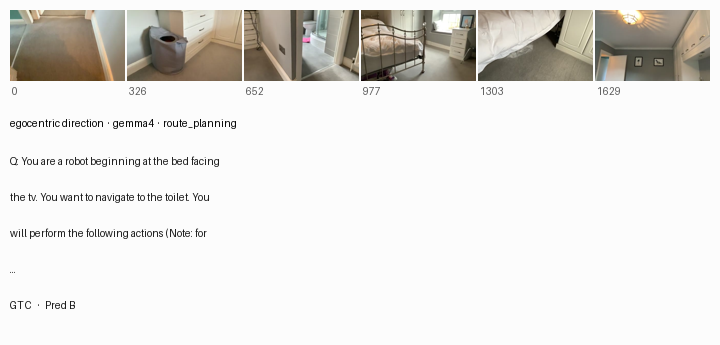
\includegraphics[width=\linewidth]{egocentric_direction_gemma4_route_planning_4959.png}
\end{minipage}\hfill
\begin{minipage}[t]{0.472\textwidth}
\centering
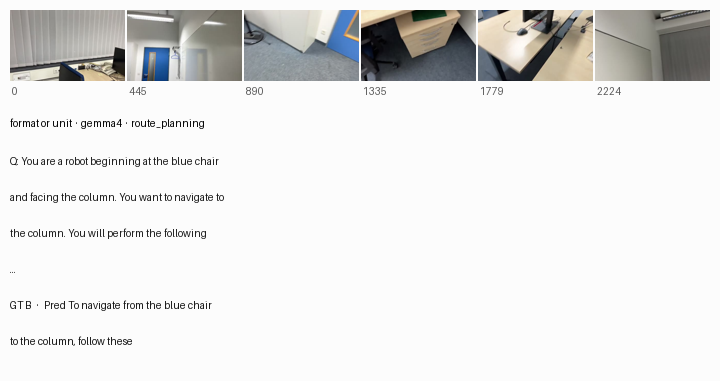
\includegraphics[width=\linewidth]{format_or_unit_gemma4_route_planning_4963.png}
\end{minipage}
\par\smallskip
\noindent
\begin{minipage}[t]{0.472\textwidth}
\centering
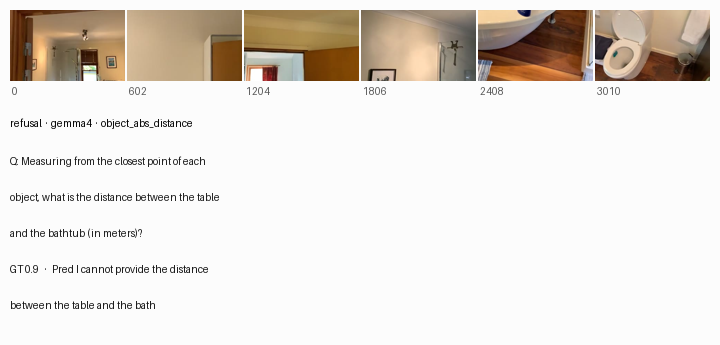
\includegraphics[width=\linewidth]{refusal_gemma4_object_abs_distance_687.png}
\end{minipage}\hfill
\begin{minipage}[t]{0.472\textwidth}
\centering
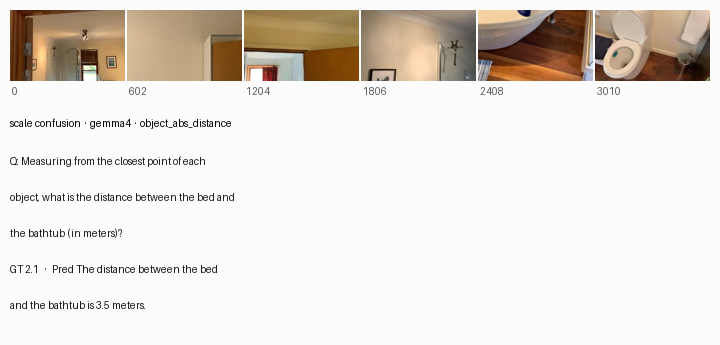
\includegraphics[width=\linewidth]{scale_confusion_gemma4_object_abs_distance_690.png}
\end{minipage}
\par\smallskip
\noindent
\begin{minipage}[t]{0.472\textwidth}
\centering
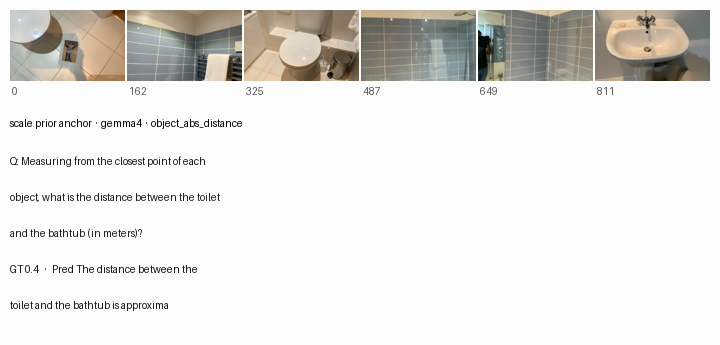
\includegraphics[width=\linewidth]{scale_prior_anchor_gemma4_object_abs_distance_684.png}
\end{minipage}
\par\smallskip

\vspace{2pt}
\begin{center}
\footnotesize\textbf{Table 2:} Failure taxonomy. Near misses inside 30\% relative error are
excluded, since MRA already gives them partial credit.\par\vspace{2pt}
{\scriptsize\begin{tabular}{@{}p{0.22\textwidth}rp{0.52\textwidth}@{}}
\toprule
Class & $n$ & Mechanism \\
\midrule
\textbf{Scale confusion} & 1824 & wrong magnitude; a prior-pinned subset sits near the task median \\
\textbf{Egocentric direction} & 378 & wrong turn sequence; B/C over-predicted, A/D under-used \\
\textbf{Refusal / abstention} & 355 & no estimate produced \\
\textbf{Answer format} & 232 & right in substance, lost to the first-token parser \\
\bottomrule
\end{tabular}}
\end{center}

\section{Discussion}
Qwen3-VL-8B is the only model of the three that measures rather than recites: 47.9 MRA on absolute distance and 57.1 on room size against 35.0 route-planning accuracy. Removing the video costs it 17.3 and 24.2 MRA points with non-overlapping intervals, yet a third of its distance score survives with no image at all, so part of any VLM's score here is prior recall in the benchmark as much as perception. Gemma-4-12B returns no room-size estimate on any of the 288 questions and needs the lenient parser to reach 22.8 on distances, so its 0.3 strict figure measures answer format, not spatial ability. Molmo2-8B tracks room size ($r{=}0.74$) but overshoots threefold, and its blind arm --- a constant 20\,m$^2$ --- sits within a point of the best constant this ground truth allows, so MRA's thresholds reward hedging; route planning, where all three converge at 29--35\%, is dominated by a letter prior rather than by failed turns. The largest remaining gain is in the input, not the model: 32 frames at 448\,px cannot carry a room's metric scale, and asking the model to verify a proposed depth or floor plan would test spatial reasoning instead of recall. The limitation is structural --- no frame budget repairs a benchmark whose numeric answers can be scored above chance by a constant.

{\scriptsize\begin{thebibliography}{9}
\footnotesize
\setlength{\itemsep}{0pt}\setlength{\parsep}{0pt}\setlength{\topsep}{2pt}
\bibitem[Yang et al.(2025)]{yang2025thinking} J.~Yang et al. \newblock Thinking in Space: How
Multimodal LLMs See, Remember and Recall Spaces. \newblock CVPR 2025. arXiv:2412.14171.
\bibitem[Model cards(2025--26)]{cards} Qwen Team; Google DeepMind; Ai2. \newblock Qwen3-VL,
Gemma 4 and Molmo 2 model cards (Hugging Face).
\bibitem[Fan et al.(2026)]{vlm3r} Z.~Fan et al. \newblock VLM-3R: Vision-Language Models
Augmented with Instruction-Aligned 3D Reconstruction. \newblock CVPR 2026.
\end{thebibliography}}

\end{document}
